% ─────────────────────────────────────────────────────────────────────────────
\chapter{PoolLiteSIS: A Lightweight Secret Image Sharing Using Pooling-Based Dimensional Reduction}
% ─────────────────────────────────────────────────────────────────────────────

This chapter presents PoolLiteSIS, a lightweight secret image sharing framework that integrates average pooling-based dimensional reduction with XOR-based share generation to achieve secure and storage-efficient distribution of images. It introduces the use of pooled representations and residual encoding, combined with image-dependent permutation for enhanced security, and details the complete pipeline for shadow generation and lossless reconstruction. The chapter further evaluates the method in terms of storage efficiency, reconstruction accuracy, and security, demonstrating significant reduction in share size while maintaining perfect reconstruction and resistance to information leakage.
\section{Introduction}

The emergence of digital multimedia content has made images a basic form of information transfer in personal, business, and scientific contexts. Many sectors prefer encoding private information in the form of images, and hence protection against unauthorized viewing and manipulation is a matter of utmost concern. Various secure measures such as encryption schemes, visual cryptographic systems, and steganographic systems have proved to be effective. Nevertheless, these techniques essentially depend on centralized storage models, which are prone to total data loss due to single-point failures. When adversaries intercept or damage the only storage device, the embedded private information becomes unrecoverable. To overcome these limitations, \textit{Secret Image Sharing (SIS)} systems use distributed storage models.

In SIS models, secure images are decomposed into several shares or shadow images, which are then shared among the participants. Only when a threshold number of shares is gathered can the image be reconstructed, while any sub-threshold collection of shares provides no information about the original image. These models are very useful in protecting highly classified information such as cryptographic keys, authorization codes, and financial data.

\section{Preliminaries}
\label{sec:lad-prelim}


This section presents the fundamental concepts and mathematical tools underlying our research framework.

\subsection{Average Pooling Operations}

Average Pooling is a form of a dimensional reduction method that is commonly used in CNN architectures. For a given input image $I$ of size $m \times n$, an average pooling operation of size $k \times k$ with a stride of $s$ divides the image into regions (possibly overlapping if $s < k$) and replaces them with their average value.

For a block $B$ of size $k \times k$, the pooled value computes as:
\begin{equation}
P_{avg} = \frac{1}{k^2}\sum_{i=1}^{k}\sum_{j=1}^{k} B_{ij}
\end{equation}

The resulting pooled image $P$ exhibits dimensions: $\frac{m}{s} \times \frac{n}{s}$. To enable perfect reconstruction, residuals are computed as:
\begin{equation}
R_{ij} = I_{ij} - P_{avg}
\end{equation}
where $R_{ij}$ captures the deviation between original pixel value $I_{ij}$ and corresponding pooled value.

\subsection{XOR-Based Secret Sharing}

The XOR operation has perfect diffusion, meaning that if one of the operands is random, the result is indistinguishable from random. We give a brief overview of the $(n,n)$ SIS scheme given by Wang et al.~\cite{wang2007}. The dealer $D$ creates $n-1$ random matrices for the $(n,n)$ threshold schemes:
\[\{B_1, B_2, \dots, B_{n-1}\}\]
Each of these matrices has the same dimensions as the secret image.

The $n$ share images $\{SI_1, SI_2, \dots, SI_n\}$ are constructed sequentially through XOR operations:
\[
SI_1 = B_1
\]
\[
SI_2 = B_1 \oplus B_2
\]
\[
SI_3 = B_2 \oplus B_3
\]
\[
\vdots
\]
\[
SI_{n-1} = B_{n-2} \oplus B_{n-1}
\]
\[
SI_n = B_{n-1} \oplus I_s
\]
where $\oplus$ denotes bitwise XOR.

To reconstruct the original image, the combiner performs bitwise XOR across all $n$ share images:
\[
I'_s = SI_1 \oplus SI_2 \oplus \dots \oplus SI_n
\]


\section{Literature Review}
\label{sec:lad-litreview}


XOR-based SIS methods were developed as computationally efficient alternatives to complex cryptographic protocols. Initial research by Wang et al.~\cite{wang2007} introduced $(n, n)$ SIS schemes in which dealers produce $(n-1)$ random matrices by computing the $n$-th share via the XOR operation of the last random matrix and the image. Share reconstruction is achieved by XORing all $n$ shares. Although removing pixel expansion and preserving perfect contrast for binary, grayscale, and color images, shadow dimensions are equal to the original images.

Later research by Chattopadhyay et al.~\cite{chattopadhyay2018} incorporated hash verification in $(n,n)$ arrangements, allowing participants to verify tampered shares before reconstruction. Although flexible when adding more shares, conventional arrangements retain the same shadow dimensions as the original images.

Chen and Wu~\cite{chen2014,chen2011} built various Multiple SIS (MSIS) schemes using Boolean operations for encoding multiple secrets into the same share sets, but with unchanged shadow dimensions. In later studies, they added more randomness to avoid partial information leakage from sub-threshold sets, but with shadows still having original dimensions. Another study by Nag et al.~\cite{nag2020} suggested Boolean MSIS schemes with individual shares expanded to $t \times r \times c$ depending on the number of secret images and the matrix arrangement. Deshmukh et al.~\cite{deshmukh2017} introduced a Chinese Remainder Theorem (CRT) method for multiple color image sharing with shadows of original sizes.

Prasetyo and Hsia~\cite{prasetyo2019improved} improved multiple secret sharing using generalized chaotic image scrambling, which combined XOR operations with hyperchaotic maps for enhanced security with reconstruction issues for odd secret numbers, but with shadows still having original dimensions. In another study~\cite{prasetyo2019lossless}, they developed lossless progressive schemes for incremental quality improvement with additional shares. Guo et al.~\cite{guo2016} suggested multi-threshold schemes using generalized CRT with shadows of original sizes.

Kabirirad and Eslami~\cite{kabirirad2018t} generalized MSIS to $(t,n)$-threshold schemes using Boolean operations, allowing flexibility where $t$ out of $n$ shares are needed for reconstruction. But this method needs $t$ consecutive shares for backtracking recovery, where the absence of any single share will disrupt the chain, and shadows retain original size. Faraoun~\cite{faraoun2020} designed highly secure $(n,n)$ multi-SIS schemes using cryptographic hash functions and stream ciphers, encrypting secrets with random session keys, then splitting keys using XOR chaining between $n$ shares, producing shadows of original size. Lin et al.~\cite{lin2024} designed key-free SIS schemes using improved Cycling-XOR techniques, embedding shares into separate cover images for better concealment, also producing shadows of original size.

Few studies focus on minimizing shadow size in XOR and Boolean schemes. Ou et al.~\cite{ou2015userfriendly} designed user-friendly secret-image sharing schemes using block truncation coding and error diffusion, resulting in shares $\frac{1}{4}$ smaller than originals, yet still meaningful. Research by Purushothama~\cite{purushothama2024} described dimensional reduction where, instead of the usual $(n,n)$-threshold XOR schemes producing shares of size $h \times w$, their scheme produces shadows of size $\lceil h/n \rceil \times w$, greatly enhancing storage space efficiency.

The literature review shows that, although XOR-based methods are simple and computationally efficient, they always produce shadows with the same dimensions as the original image ($n \times n$), which results in high redundancy and storage costs. The focus of research has been on improving security, but not on the limitations of storage efficiency. This chapter proposes to maintain the advantages of lightweight and lossless XOR operations while significantly reducing the shadow size by using pooling-based dimensional reduction and permutation techniques based on images.


\section{Work Done}
\label{sec:lad-work}
% ─────────────────────────────────────────────────────────────────────────────
The basic problem in SIS is to strike a balance between security, reconstruction accuracy, and storage space efficiency. The existing approaches tend to focus on security with the penalty of storage space overhead. The contributions of this research work are as follows:

\begin{enumerate}
\item We propose a new XOR-based SIS framework that combines average pooling to achieve 75\% spatial dimension reduction, significantly reducing the sizes of shadow images.

\item We describe a secure residual permutation technique using the pooled image as a seed, making it impossible to leverage the residual information without having the entire shadow image.

\item We show a total storage reduction of 75\% for shadow images over traditional XOR-based approaches while ensuring perfect lossless reconstruction.

\item We offer a thorough experimental evaluation on standard benchmark images, examining both storage and security properties.
\end{enumerate}

\begin{figure}[H]
\centering
\begin{tikzpicture}[
node distance=0.4cm and 0.4cm,
block/.style={rectangle, draw, text width=2.2cm, align=center, font=\small},
scale=0.8, transform shape
]

  \node[block] (secret)
    {Secret Image S};

  \node[block, below=of secret] (pool)
    {Average Pooling:\\Generate P and R};

  \node[block, below left=0.4cm and 0.5cm of pool] (xor)
    {XOR Shadow Generation:\\Create $n$ shadows};

  \node[block, below right=0.4cm and 0.5cm of pool] (permute)
    {Permute Residuals\\using P as seed};

  \node[block, below=1.4cm of pool] (dist)
    {Distribution of shadows};

  \node[block, below=of dist] (recon)
    {Reconstruction:\\XOR + unpermute};

  \node[block, below=of recon] (recovered)
    {Recovered Image};

  \draw[->] (secret) -- (pool);
  \draw[->] (pool) -- (xor);
  \draw[->] (pool) -- (permute);
  \draw[->] (xor) -- (dist);
  \draw[->] (permute) -- (dist);
  \draw[->] (dist) -- (recon);
  \draw[->] (recon) -- (recovered);

\end{tikzpicture}
\caption{Comprehensive Overview of Proposed Framework}
\label{fig:methodology}
\end{figure}


Our system consists of three major stages: preprocessing by average pooling, shadow creation by cyclic XOR operations, and reconstruction by unpooling. First, the secret image $S$ is subjected to \textit{average pooling}, resulting in two complementary parts: the pooled matrix $P$ and the residual matrix $R$. The pooled matrix $P$ serves as a compact form, later used to produce multiple shadows based on XOR operations. At the same time, the residuals $R$ are subjected to \textit{permutation with $P$ as the seed}, making sure that the reconstruction key is image-dependent and cannot be reverse-engineered by unauthorized parties. In the \textit{distribution phase}, the produced shadows are safely distributed among the shareholders. To restore the original secret image, all shadows are subjected to XOR operations, and the residuals are \textit{unpermuted with the same seed $P$}. This produces the restored secret image, which retains perfect visual quality without losing any information. Our system is designed to produce shadows with a considerably smaller size, with a maximum reduction of 75\% compared to the original secret image, outperforming other XOR-based techniques. The entire processing chain is shown in Figure \ref{fig:methodology}.

\subsection{Phase 1: Average Pooling Preprocessing}

The pooling operation divides the original grayscale image \(S \in \mathbb{R}^{N \times N}\) into non-overlapping blocks of size \(K \times K\). Let \(s\) be the stride (for non-overlapping blocks, usually \(s = K\)). For each block \((i,j)\), the pooled value \(P(i,j)\) is defined as the arithmetic mean of the \(K^2\) pixel values in that block:
\[
P(i,j)\;=\;\frac{1}{K^2}\sum_{x=i\cdot s}^{(i+1)\cdot s-1}\sum_{y=j\cdot s}^{(j+1)\cdot s-1} S(x,y).
\]

The residual map \(R\in\mathbb{R}^{N\times N}\) captures per-pixel deviations from block averages:
\[
R(x,y)\;=\;S(x,y)\;-\;P\Big(\Big\lfloor\frac{x}{s}\Big\rfloor,\Big\lfloor\frac{y}{s}\Big\rfloor\Big).
\]

Since \(R\) maintains identical spatial dimensions as \(S\), the original image can be reconstructed exactly (in exact arithmetic) by adding the block-wise broadcast of \(P\) to \(R\):
\[
\widehat{S}(x,y)\;=\;P\Big(\Big\lfloor\frac{x}{s}\Big\rfloor,\Big\lfloor\frac{y}{s}\Big\rfloor\Big)\;+\;R(x,y).
\]

The pooling process is summarized in Algorithm~\ref{alg:avg_pooling}. This phase generates the following outputs:

\begin{enumerate}
\item \textbf{Pooled Image} $P$: A dimensionally reduced version of size $N/s \times N/s$ pixels, where $s$ is the pooling stride.
\item \textbf{Residual Image} $R$: A matrix of size $N \times N$ storing the difference between each original pixel and its corresponding pooled average value.
\end{enumerate}

Note that, in practice, when storing \(P\) as an integer type (e.g., \texttt{uint8}), the block mean is typically rounded (e.g., to nearest integer or truncated). This introduces a quantization error, which can be compensated for by the residuals (if stored with sufficient precision). If the residuals are stored as signed integers with sufficient range, then exact reconstruction is still possible even if \(P\) is rounded, as long as the rounding strategy is consistent during pooling and unpooling operations.

\begin{algorithm}[H]
\caption{Average Pooling}
\label{alg:avg_pooling}
\LinesNumbered

\KwIn{Grayscale image $S$ of size $N \times N$, pooling window of size $K \times K$, stride $s$}
\KwOut{Pooled image $P$ of size $\frac{N}{s} \times \frac{N}{s}$ and residual image $R$ of size $N \times N$}

$P \gets$ zero matrix of size $\frac{N}{s} \times \frac{N}{s}$

$R \gets$ zero matrix of size $N \times N$

\vspace{4pt}
\For{$i \gets 0$ \textbf{to} $\frac{N}{s}-1$}{
    \For{$j \gets 0$ \textbf{to} $\frac{N}{s}-1$}{
        Extract block $B \gets S[i \cdot s : (i+1) \cdot s, \; j \cdot s : (j+1) \cdot s]$ \\
        Compute block average $a \gets \text{mean}(B)$ \\
        Assign pooled value $P(i, j) \gets a$ \\
        Compute residuals: \\
        $R[i \cdot s : (i+1) \cdot s, \; j \cdot s : (j+1) \cdot s] \gets B - a$
    }
}

\Return $P, R$
\end{algorithm}

\subsection*{Illustrative Example: $4\times4$ Image with $2\times2$ Pooling (Block Size $K=2$, Stride $s=2$)}

Consider input image \(S\) as the \(4\times4\) matrix:
\[
S =
\begin{bmatrix}
100 & 102 & 50 & 52 \\
98  & 101 & 49 & 51 \\
200 & 202 & 150 & 151 \\
198 & 199 & 149 & 152
\end{bmatrix}.
\]

We partition \(S\) into four non-overlapping \(2\times2\) blocks. Computing block sums and means:

\begin{itemize}
  \item Top-left block (index \((0,0)\)):
    \[
    B_{00} = \begin{bmatrix}100 & 102\\ 98 & 101\end{bmatrix},
    \quad
    \text{sum}(B_{00})=401,
    \quad  
    P(0,0)=100.25.
    \]
  \item Top-right block (index \((0,1)\)):
    \[
    B_{01} = \begin{bmatrix}50 & 52\\ 49 & 51\end{bmatrix},
    \quad
    \text{sum}(B_{01})=202,
    \quad
    P(0,1)=50.5.
    \]
  \item Bottom-left block (index \((1,0)\)):
    \[
    B_{10} = \begin{bmatrix}200 & 202\\ 198 & 199\end{bmatrix},
    \quad
    \text{sum}(B_{10})=799,
    \quad
    P(1,0)=199.75.
    \]
  \item Bottom-right block (index \((1,1)\)):
    \[
    B_{11} = \begin{bmatrix}150 & 151\\ 149 & 152\end{bmatrix},
    \quad
    \text{sum}(B_{11})=602,
    \quad
    P(1,1)=150.5.
    \]
\end{itemize}

Thus the pooled image \(P\) (size \(2\times2\)) becomes:
\[
P = \begin{bmatrix}
100.25 & 50.5 \\
199.75 & 150.5
\end{bmatrix}.
\]

Next, we compute the full-size residual map \(R\) by subtracting corresponding block means from each pixel:

Top-left residuals for block \(B_{00}\):
\[
\begin{array}{cc}
R(0,0)=-0.25, & R(0,1)=1.75,\\[4pt]
R(1,0)=-2.25,  & R(1,1)=0.75.
\end{array}
\]

Top-right residuals for \(B_{01}\):
\[
\begin{array}{cc}
R(0,2)=-0.5, & R(0,3)=1.5,\\[4pt]
R(1,2)=-1.5,  & R(1,3)=0.5.
\end{array}
\]

Bottom-left residuals for \(B_{10}\):
\[
\begin{array}{cc}
R(2,0)=0.25, & R(2,1)=2.25,\\[4pt]
R(3,0)=-1.75, & R(3,1)=-0.75.
\end{array}
\]

Bottom-right residuals for \(B_{11}\):
\[
\begin{array}{cc}
R(2,2)=-0.5, & R(2,3)=0.5,\\[4pt]
R(3,2)=-1.5,  & R(3,3)=1.5.
\end{array}
\]

Collecting these entries yields the residual matrix:
\[
R =
\begin{bmatrix}
-0.25 & 1.75  & -0.5 & 1.5 \\
-2.25 & 0.75  & -1.5 & 0.5 \\
0.25  & 2.25  & -0.5 & 0.5 \\
-1.75 & -0.75 & -1.5 & 1.5
\end{bmatrix}.
\]

\subsection{Phase 2: Residual Permutation for Security}

\begin{algorithm}[H]
\caption{Permutation of Residual Matrix}
\label{alg:residual_permutation}
\LinesNumbered
\setcounter{AlgoLine}{0}

\KwIn{Residual matrix $R$ of size $N \times N$, pooled image $P$}
\KwOut{Permuted residual matrix $R'$ and permutation indices $\pi$} 

Compute the seed value from the pooled image: \\
$s \gets \left( \sum_{i=1}^{N} \sum_{j=1}^{N} P(i,j) \right) \bmod 2^{32}$ \\

Initialize pseudo-random generator using $s$\;

Flatten $R$ into vector $R_f$ of length $M = N \times N$\;

Create index vector $I \gets [0, 1, \dots, M-1]$\;

Randomly shuffle $I$ using the initialized generator to obtain $\pi$\;

\For{$k \gets 0$ \KwTo $M-1$}{
    $R'_f[k] \gets R_f[\pi[k]]$\;
} 

Reshape $R'_f$ into $R'$ of size $N \times N$\;

\Return $R', \pi$\;
\end{algorithm}

A major security issue arises when the residual image $R$, without being permuted, tends to be similar to the original image $S$. The unpermuted residuals had relatively high SSIM values with the pooled image, signifying a leakage of information. To maintain confidentiality, the residual matrix is permuted through a deterministic pseudo-random permutation generated from the pooled image itself. This involves:

\begin{itemize}
    \item \textbf{Seed generation}: A unique seed $s$ is computed from the pixel intensities of the pooled image as:
\[
s = \left( \sum_{i=1}^{M} \sum_{j=1}^{N} P(i,j) \right) \bmod 2^{32}
\]
This seed initializes a random number generator, ensuring that the permutation is image-dependent and reproducible only after reconstructing the pooled image from all secret shares.

\item \textbf{Permutation:}
Let the flattened residual vector be $R_f = [r_0, r_1, \dots, r_{N-1}]$ where $N = M \times N$.  
A random permutation vector $\pi = [\pi(0), \pi(1), \dots, \pi(N-1)]$ is generated, and the permuted residuals are obtained as:
\[
R'_f[i] = R_f[\pi(i)], \quad \forall i \in [0, N-1]
\]
Finally, $R'_f$ is reshaped to form the permuted residual matrix $R'$.

\end{itemize}

This process provides the benefit of implicitly securing the permutation key, thereby obviating the need for key exchange. Algorithm \ref{alg:residual_permutation} illustrates the procedure adopted to permute the residual image. After the permutation process, the SSIM value between the permuted residuals and the pooled image decreases substantially, thereby destroying the structural correlations.

\subsection{Phase 3: Cyclic XOR-Based Shadow Construction}

This stage uses the XOR-based SIS method, where the cyclic XOR operations are employed to create the shadow images. This is done by taking advantage of the basic property of the XOR operation, which is its own inverse, as expressed below:
\[
A \oplus B \oplus B = A
\]

This property ensures that when two XOR operations are carried out using the same operand, the presence of the operand is completely eliminated. Therefore, it becomes possible to divide the information into several shadow images, where each shadow image holds a part of the total information, and the original pooled image $P$ can only be reconstructed if all $n$ shadow images are obtained.


\begin{algorithm}[H]
\small
\caption{XOR-Based Shadow Generation}
\label{alg:cyclic_xor}
\LinesNumbered
\setcounter{AlgoLine}{0}

\KwIn{Pooled image $I_s = P$ of size $\frac{N}{s} \times \frac{N}{s}$}
\KwIn{Stride $s$, number of shadows $n$}

\KwOut{Shadow set $\{SI_1, SI_2, \dots, SI_n\}$}

$M \gets \frac{N}{s}$\;
Spatial dimension of pooled image\;

\For{$i = 1$ \KwTo $n-1$}{
    Generate random matrix $B_i$\;
    Size: $M \times M$, values in $[0,255]$\;
}

$SI_1 \gets B_1$\;

\For{$i = 2$ \KwTo $n-1$}{
    $SI_i \gets B_{i-1} \oplus B_i$\;
}

$SI_n \gets B_{n-1} \oplus I_s$\;

\Return $\{SI_1, SI_2, \dots, SI_n\}$\;

\end{algorithm}


Let $I_s = P$ be the pooled image formed after the average pooling phase, with a size of $\frac{N}{s} \times \frac{N}{s}$. To form the $n$ shadow images, the dealer first creates $n-1$ random matrices $\{B_1, B_2, \ldots, B_{n-1}\}$ of the same size as $I_s$. Each $B_i$ is populated with random grayscale values uniformly distributed between the range $[0, 255]$, thus removing any recognizable pattern of the original image.

The shadow images $\{SI_1, SI_2, \ldots, SI_n\}$ are created through a cyclic XOR operation sequence. The dealer first assigns the first random matrix as the first shadow image and then applies a cyclic XOR operation between consecutive random matrices to form the subsequent shadow images. The last shadow image combines the last random matrix with the pooled image, thus hiding the secret message inside the cyclic XOR operation chain. The expression for the resulting formulation is as follows:
\begin{align}
SI_1 &= B_1 \nonumber \\
SI_2 &= B_1 \oplus B_2 \nonumber \\
SI_3 &= B_2 \oplus B_3 \nonumber \\
&\vdots \nonumber \\
SI_{n-1} &= B_{n-2} \oplus B_{n-1} \nonumber \\
SI_n &= B_{n-1} \oplus I_s \nonumber
\end{align}

A pseudocode implementation of this is shown in Algorithm \ref{alg:cyclic_xor}. The shadow images are of the same size as the pooled image of $\frac{N}{s} \times \frac{N}{s}$, which is 75\% smaller than the original secret image in the case of K=s=2.


\subsection{Phase 4: Reconstruction}
Algorithm \ref{alg:reconstruction} summarizes the steps to recover the secret image after obtaining all the share images.


To recover the secret image, the combiner performs the following steps:


\begin{enumerate}
\item \textbf{XOR all shadow images} to reconstruct the pooled image:
\begin{equation}
I'_s = SI_1 \oplus SI_2 \oplus \ldots \oplus SI_n = P
\end{equation}

Due to the cyclic cancellation property of XOR, all random matrices cancel out, leaving only the pooled image.

\item \textbf{Reverse the permutation} using $I'_s$ as the seed to generate the permutation matrix $\pi$, then compute:
\begin{equation}
R = \pi^{-1}(R_{permuted})
\end{equation}

\item \textbf{Apply average unpooling}: Upsample the pooled image by replicating each value to fill its corresponding $K \times K$ block, then add the residuals:
\begin{equation}
S_{ij} = P'_{avg} + R_{ij}
\end{equation}

This process guarantees perfect reconstruction of the original secret image.
\end{enumerate}

\begin{algorithm}[H]
\small
\caption{Reveal Phase}
\label{alg:reconstruction}
\LinesNumbered
\setcounter{AlgoLine}{0}

\KwIn{Shadow set $\{SI_1, SI_2, \dots, SI_n\}$}
\KwIn{Permuted residuals $R_{\text{permuted}}$, stride $s$}

\KwOut{Reconstructed image $I_{\text{reconstructed}}$}

$I_s \gets SI_1$\;

\For{$i = 2$ \KwTo $n$}{
    $I_s \gets I_s \oplus SI_i$\;
}

Compute seed from $I_s$\;
$seed\_value \gets \sum_{i,j} I_s(i,j)$\;
$seed\_value \gets seed\_value \bmod 2^{32}$\;

Initialize PRNG with $seed\_value$\;

Generate permutation vector $\pi$\;

$R' \gets R_{\text{permuted}} - 128$\;

$R \gets \pi^{-1}(R')$\;

\For{$p = 0$ \KwTo $\frac{N}{s} - 1$}{
    \For{$q = 0$ \KwTo $\frac{N}{s} - 1$}{
        \For{$a = 0$ \KwTo $s - 1$}{
            \For{$b = 0$ \KwTo $s - 1$}{
                $x \gets ps + a$\;
                $y \gets qs + b$\;
                $I_{\text{reconstructed}}[x,y] \gets I_s[p,q] + R[x,y]$\;
            }
        }
    }
}

\Return $I_{\text{reconstructed}}$\;

\end{algorithm}

% ─────────────────────────────────────────────────────────────────────────────
\section{Results and Analysis}
\label{sec:lad-results}


We have validated our proposed approach using n = 4 shadows, and we have created a (4, 4) threshold configuration. The standard grayscale Cameraman image with 512 × 512 pixels was used as our test image. All experiments were performed using Python 3.8, and NumPy was used for matrix calculations.

\subsection{Storage Efficiency Analysis}

Table~\ref{tab:storage_analysis} presents a comparative analysis of storage requirements between our approach and a conventional XOR-based (4, 4) scheme without pooling.

\begin{table}[h!]
\centering
\caption{Storage Analysis: Proposed Method vs. Naive XOR Scheme}
\label{tab:storage_analysis}
\begin{tabular}{|l|c|}
\hline
\textbf{Component} & \textbf{Size (bytes)} \\ \hline
Original Image & 262,144 \\ \hline
\multicolumn{2}{|c|}{\textit{Naive XOR Scheme}} \\ \hline
Individual Share Size & 262,144 \\ 
Total Storage (4 shares) & 1,048,576 \\ \hline
\multicolumn{2}{|c|}{\textit{Proposed Method}} \\ \hline
Individual Share Size & 65,536 \\ 
Total Storage (4 shares) & 262,144 \\ \hline
\textbf{Storage Reduction} & \textbf{75.00\%} \\ \hline
\end{tabular}
\end{table}

\begin{itemize}
\item The traditional XOR method needs to store 1,048,576 bytes (1024 KB) because each of the four shadow images has the same size as the original image, which is 256 KB.

\item Our proposed method only needs to store 262,144 bytes (256 KB) in total, which is 4 × 65,536 = 262,144 bytes for the four shadow images.

\item This brings a 75\% reduction in the total storage needs while providing the same level of security guarantees.
\end{itemize}

\subsection{Reconstruction Quality}

Perfect lossless reconstruction was obtained in all experiments. Table~\ref{tab:quality_metrics} shows the quality measures for each test image. The infinite PSNR value and SSIM of 1.0 indicate that the reconstructed images are pixel-perfect copies of the original secret images with no loss of information.

\begin{table}[h!]
\centering
\caption{Reconstruction Quality Metrics}
\label{tab:quality_metrics}
\begin{tabular}{|l|c|c|}
\hline
\textbf{Image} & \textbf{PSNR (dB)} & \textbf{SSIM} \\ \hline
Jet & $\infty$ & 1.0000 \\ \hline
Cameraman & $\infty$ & 1.0000 \\ \hline
Milk & $\infty$ & 1.0000 \\ \hline
Baboon & $\infty$ & 1.0000 \\ \hline
Barbara & $\infty$ & 1.0000 \\ \hline
Bridge & $\infty$ & 1.0000 \\ \hline
\end{tabular}
\end{table}

\subsection{Security Validation}

We calculated the Structural Similarity Index (SSIM) among various components to check the security of the residual permutation. Table~\ref{tab:security_validation} presents the security analysis of the Cameraman image. The most important points to note are:

\begin{itemize}
\item The unpermuted residuals are highly similar (SSIM $\approx$ 0.79--0.85) to the combined image, which may lead to leakage of information.

\item However, after permutation, the similarity reduces significantly to 0.03, which ensures the removal of structural information.

\item The individual shadow images do not contain any information about the secret, as their similarity (SSIM $\approx$ 0.01-0.02) to the original and combined images is very low.
\end{itemize}

\begin{table}[h!]
\centering
\caption{SSIM Analysis for Security Validation (Cameraman Image)}
\label{tab:security_validation}
\begin{tabular}{|l|c|}
\hline
\textbf{Comparison} & \textbf{SSIM} \\ \hline
Permuted Residuals vs. Original Image & 0.03 \\ \hline
Individual Shadow vs. Pooled Image & 0.01 \\ \hline
\end{tabular}
\end{table}

\subsection{Computational Complexity}

The computational complexity of our method is dominated by:

\begin{enumerate}
\item \textbf{Pooling Operation}: $O(mn)$ for an $m \times n$ image
\item \textbf{Permutation}: $O(mn)$ for generating and applying the permutation
\item \textbf{XOR Operations}: $O(n \cdot \frac{m}{k} \cdot \frac{n}{k})$ for $n$ shadows on a pooled image
\item \textbf{Unpooling}: $O(mn)$ for reconstruction
\end{enumerate}

All operations are linear in image size, ensuring efficiency for real-world applications. XOR operations are especially fast because of bitwise parallelism in modern processors.

\subsection{Visual Results}

Figure~\ref{fig:test_image_cameraman} shows the standard benchmark image used in our experiments. The Cameraman image is suitable for testing the effectiveness of the proposed method because of the presence of both smooth and textured areas.

\begin{figure}[H]
\centering
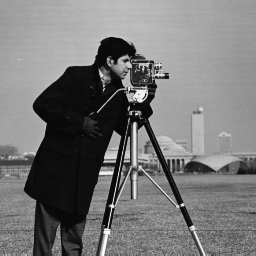
\includegraphics[width=0.4\textwidth]{images/cameraman.png}
\caption{Cameraman image ($512 \times 512$) used as the test image for evaluation.}
\label{fig:test_image_cameraman}
\end{figure}

Figure~\ref{fig:xor_full_pipeline} shows the overall process of our proposed XOR-based technique with pooling and permutation for the Cameraman image. The figure clearly shows the transition from the original secret image to the four shadow images after the creation of residuals and permutation. The shadow images, which look like noise, ensure that there is no leakage of information about the secret image. The noise nature of the permuted residuals proves that the permutation technique is effective in removing structural information.

\begin{figure}[H]
\centering

% Row 1: Original and Permuted Residuals
\subfloat[Original Image]{%
    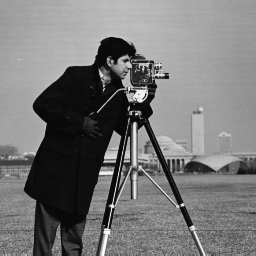
\includegraphics[width=0.4\textwidth]{images/cameraman.png}%
    \label{fig:Cameraman_orig}}%
\hfill
\subfloat[Permuted Residuals]{%
    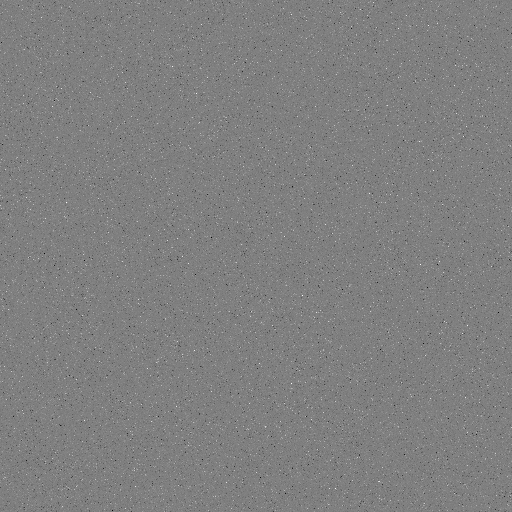
\includegraphics[width=0.4\textwidth]{images/xor-pooling/lena-xor-permuted-residuals.png}%
    \label{fig:Cameraman_permuted}}%

\vspace{0.5cm}

% Row 2: Four Shadow Images
\subfloat[Shadow Image 1]{%
    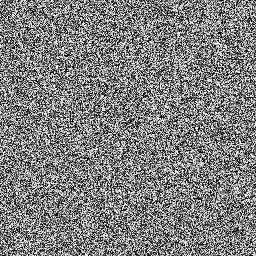
\includegraphics[width=0.22\textwidth]{images/xor-pooling/lena-xor-share1.png}%
    \label{fig:lena_shadow1}}%
\hfill
\subfloat[Shadow Image 2]{%
    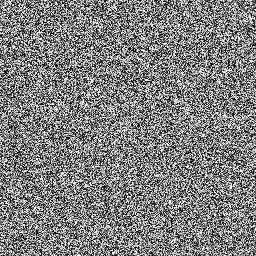
\includegraphics[width=0.22\textwidth]{images/xor-pooling/lena-xor-share2.png}%
    \label{fig:lena_shadow2}}%
\hfill
\subfloat[Shadow Image 3]{%
    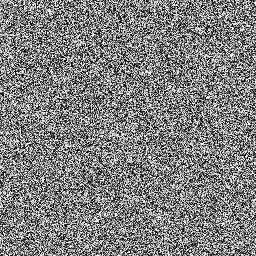
\includegraphics[width=0.22\textwidth]{images/xor-pooling/lena-xor-share3.png}%
    \label{fig:lena_shadow3}}%
\hfill
\subfloat[Shadow Image 4]{%
    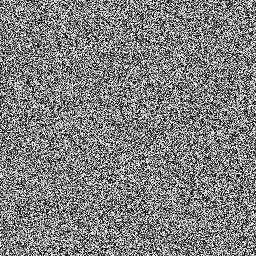
\includegraphics[width=0.22\textwidth]{images/xor-pooling/lena-xor-share4.png}%
    \label{fig:lena_shadow4}}%

\caption{Visual demonstration of the pooling-permutation optimized XOR-based SIS pipeline on the Cameraman image. 
(a) Original $512 \times 512$ secret image. 
(b) Permuted residuals showing destroyed structural correlation (SSIM = 0.03). 
(c–f) Four shadow images of size $256 \times 256$ appearing as random noise.}
\label{fig:xor_full_pipeline}
\end{figure}

Moreover, Figure~\ref{fig:cameraman_reconstruction_comparison} illustrates the reconstruction attempts with only three out of the four shares and two out of the four shares on the Cameraman test image. The reconstructed images are obviously noisy and do not have any resemblance to the original hidden image. This verifies that our scheme satisfies the basic requirement of SIS, which is that no information is revealed with less than the threshold number of shares.

\begin{figure}[H]
\centering

% Row 1: Original, 2-share, and 3-share Reconstruction
\subfloat[Original Image]{%
    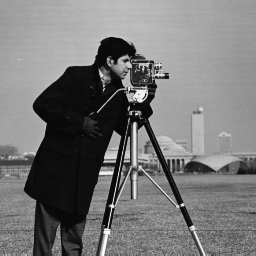
\includegraphics[width=0.3\textwidth]{images/cameraman.png}%
    \label{fig:cameraman_orig2}}%
\hfill
\subfloat[Reconstructed Image with any 2 Shares]{%
    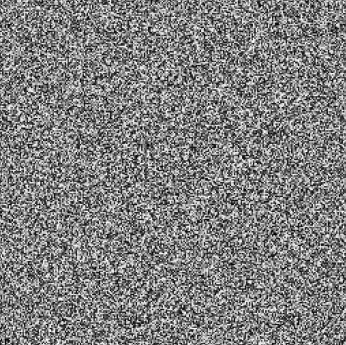
\includegraphics[width=0.3\textwidth]{images/failed_reconstructions/failed_2share.png}%
    \label{fig:cameraman_2share}}%
\hfill
\subfloat[Reconstructed Image with any 3 Shares]{%
    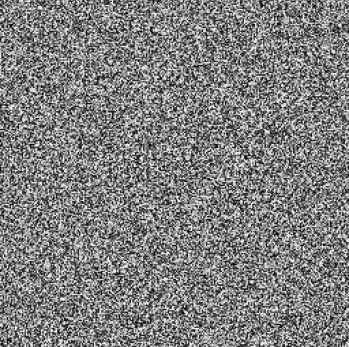
\includegraphics[width=0.3\textwidth]{images/failed_reconstructions/baboon_3share_reconstruction.png}%
    \label{fig:cameraman_3share}}%

\vspace{0.5cm}

% Row 2: Four Shadow Images
\subfloat[Shadow Image 1]{%
    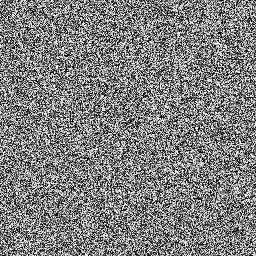
\includegraphics[width=0.22\textwidth]{images/xor-pooling/lena-xor-share1.png}%
    \label{fig:cameraman_shadow1}}%
\hfill
\subfloat[Shadow Image 2]{%
    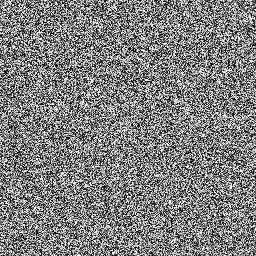
\includegraphics[width=0.22\textwidth]{images/xor-pooling/lena-xor-share2.png}%
    \label{fig:cameraman_shadow2}}%
\hfill
\subfloat[Shadow Image 3]{%
    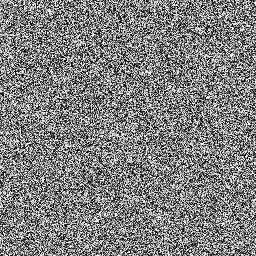
\includegraphics[width=0.22\textwidth]{images/xor-pooling/lena-xor-share3.png}%
    \label{fig:cameraman_shadow3}}%
\hfill
\subfloat[Shadow Image 4]{%
    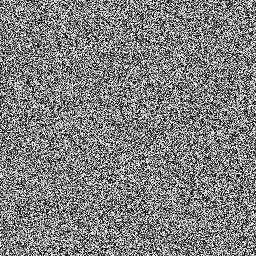
\includegraphics[width=0.22\textwidth]{images/xor-pooling/lena-xor-share4.png}%
    \label{fig:cameraman_shadow4}}%

\caption{Comparison between the original Cameraman image and its partial reconstructions using different numbers of shares.
(a) Original $512 \times 512$ secret image. 
(b) Reconstruction from any 2 shares showing complete information loss.
(c) Reconstruction from any 3 shares showing complete information loss.
(d–g) Corresponding four shadow images (each $256 \times 256$) appearing as random noise.}
\label{fig:cameraman_reconstruction_comparison}
\end{figure}

\subsection{Storage Analysis with Varying Number of Shares}

We analyzed the storage requirements for n = 2 to 10 to determine the scalability of the proposed secure pooling-based sharing system with the number of shares n. The original grayscale image was 512 × 512 pixels, which corresponds to an initial storage capacity of 262,144 bytes.

Our scheme decomposes the image into a pooled image reduced by a factor of two and a residual matrix. Although the residual matrix is stored separately, the pooled image is shared by all participants. The storage analysis does not include the residual matrix in the total storage computation.

Thus, the total storage is comprised entirely of all pooled shares. This corresponds to a 75% reduction in storage over the storage required for n complete copies of the original image. Table~\ref{tab:storage_varying_n} below summarizes the total storage computation for various values of n.

\begin{table}[H]
\centering
\tiny
\setlength{\tabcolsep}{6pt} 
\renewcommand{\arraystretch}{0.9}
\caption{Total storage requirements for different number of shares ($n$), excluding the residual matrix.}
\label{tab:storage_varying_n}
\begin{tabular}{|r|r|r|r|r|r|r|}
\hline
\textbf{$n$} & \textbf{Original (B)} & \textbf{Pooled (B)} & \textbf{Per Share (B)} & \textbf{Total (B)} & \textbf{Naive Total (B)} & \textbf{Reduction (\%)} \\
\hline
2  & 262144 & 65536 & 65536 & 131072 & 524288 & 75.00 \\
3  & 262144 & 65536 & 65536 & 196608 & 786432 & 75.00 \\
4  & 262144 & 65536 & 65536 & 262144 & 1048576 & 75.00 \\
5  & 262144 & 65536 & 65536 & 327680 & 1310720 & 75.00 \\
6  & 262144 & 65536 & 65536 & 393216 & 1572864 & 75.00 \\
7  & 262144 & 65536 & 65536 & 458752 & 1835008 & 75.00 \\
8  & 262144 & 65536 & 65536 & 524288 & 2097152 & 75.00 \\
9  & 262144 & 65536 & 65536 & 589824 & 2359296 & 75.00 \\
10 & 262144 & 65536 & 65536 & 655360 & 2621440 & 75.00 \\
\hline
\end{tabular}
\end{table}

\begin{figure}[H]
\centering
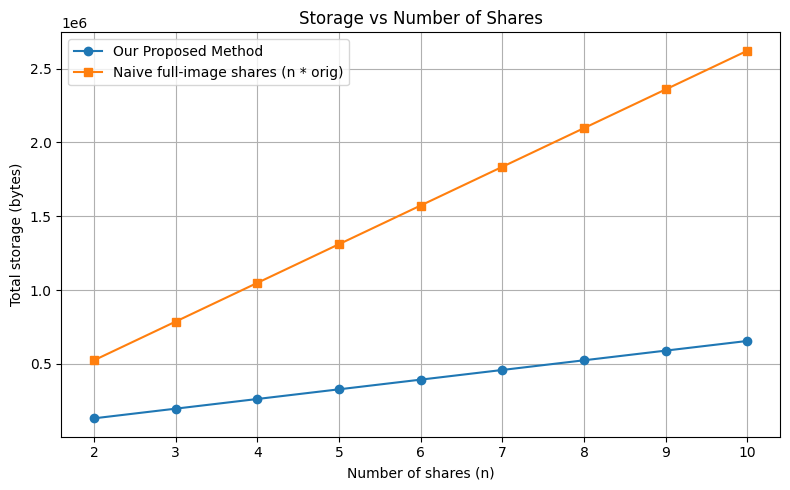
\includegraphics[width=0.7\textwidth]{images/storage_plot_1.png}
\caption{Comparison of secure and naive total storage with increasing number of shares.}
\label{fig:storage_plot}
\end{figure}

For example, when n = 4, the contribution of each of the four pooled shares to the storage is 262,144 bytes. On the other hand, the naive approach of full-image sharing would have resulted in the storage of 1,048,576 bytes, resulting in a 75\% reduction. Figure~\ref{fig:storage_plot} plots the storage comparison graphically for varying numbers of shares.

In general, the results clearly show that the secure pooling-based approach maintains perfect reconstruction with substantial storage savings. The storage savings are constant at 75\% for any value of n, clearly indicating the efficiency of the pooled shares in storage.

\subsection{Comparison with Existing XOR-Based Methods}

The performance of the proposed pooling-based XOR SIS approach is compared with other existing XOR-based methods reported in the literature. The comparison is highlighted in Table~\ref{tab:xor_comparison}.

\begin{table*}[htbp]
\centering
\caption{Comparison between a few XOR-based SIS schemes}
\label{tab:xor_comparison}
\resizebox{\textwidth}{!}{%
\begin{tabular}{@{}lcccc@{}}
\toprule
\textbf{Schemes} & \textbf{Lossless recovery} & \textbf{Share type} & \textbf{Access structure} & \textbf{Share size} \\ 
\midrule
Wang \textit{et al.}~\cite{wang2007} scheme-2 & yes & meaningless & (n, n) & $n \times n$ \\
Chen–Wu~\cite{chen2011,chen2014} & yes & meaningless & (n, n) & $n \times n$ \\
Lin \textit{et al.}~\cite{lin2024} & yes & meaningless & (n, n) & $n \times n$ \\
Guo \textit{et al.}~\cite{guo2016} & yes & meaningless & (t, n) & $n \times n$ \\
Prasetyo-Hsia~\cite{prasetyo2019lossless} & conditional & meaningless & (n, n) progressive & $n \times n$ \\
Chattopadhyay \textit{et al.}~\cite{chattopadhyay2018} & yes & meaningless & (n, n) & $n \times n$ \\
Faraoun~\cite{faraoun2020} & yes & meaningless & (n, n) & $n \times n$ \\
Chattopadhyay \textit{et al.}~\cite{chattopadhyay2022efficient} & yes & meaningless & (t, n) & $n \times n$ \\
Kabirirad-Eslami~\cite{kabirirad2018t,kabirirad2019verifiable} & yes & meaningless & (t, n) & $n \times n$ \\
Soreng and Kandar~\cite{soreng2023} & yes & meaningless & (t, n) & $n \times n$ \\ 
\midrule
\textbf{Our proposed method} & \textbf{yes} & \textbf{meaningless} & \textbf{(n, n)} & $\bm{\frac{n}{4} \times \frac{n}{4}}$ \\
\bottomrule
\end{tabular}%
}
\end{table*}

\section{Summary}

The proposed SIS method shows a substantial improvement over the existing XOR-based methods by realizing a 75\% reduction in total storage needs without compromising the quality of reconstruction. The experimental results on the test images validate that the reconstructed output preserves the lossless fidelity with PSNR = $= \infty$ and SSIM = 1.0. The addition of the residual permutation mechanism further improves the security by shattering the structural relationships, which is evident from the low SSIM values between the residual and pooled images, thus indicating the negligible information disclosure.